\section{Development and Implementation of the Calibration Source}

\subsection{Tritiated Methane Removal}
\label{sec:RD}

The removal efficiency of zirconium getters for methane in xenon had previously been studied at the University of Maryland.  It was found that greater than 99.99\% of natural methane can be removed in a single pass through a zirconium getter. \cite{Dobi} Tritiated methane is chemically identical to natural methane, so it follows that similar removal efficiencies should be expected for CH$_3$T.  To verify this a small scale tritiated methane injection system was integrated into a liquid xenon system at the University of Maryland.  This system used a SAES MC1-905F methane purifier placed in series immediately after the CH$_3$T source bottle to prevent non-methane species of tritium from entering the plumbing. Over 68,000 Bq of observed CH$_3$T activity was injected into this small scale system and a removal efficiency of over 99.99\% for tritiated methane in xenon was confirmed.

\begin{figure}[h!]\centering
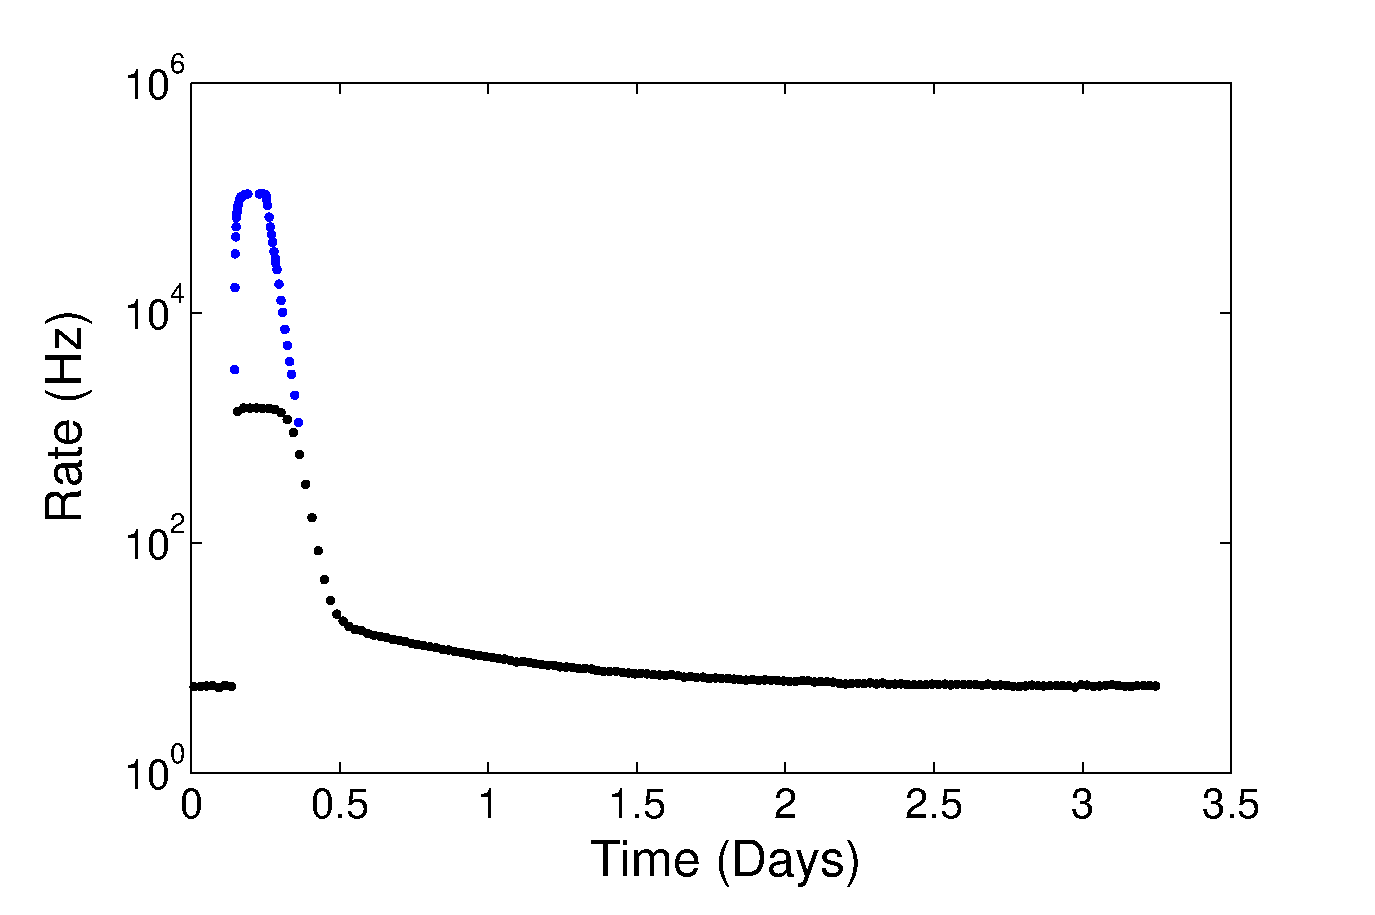
\includegraphics[width=80mm]{TimeHisto_Analog2.eps}
\caption{A time histogram of the event rate during a tritium injection into our small scale detector. The event rate greatly exceeded the limits of our ADC (black data points), so a analog scalar was used to count the true event rate (blue data points). }
\label{fig:Density}
\end{figure}


The liquid system was also used to study the effect of out gassing from plastics on the residual background rate after a CH$_3$T injection.  We found that the addition of plastic curtains around our PMTs does not impair our ability to remove CH$_3$T at $>$ 99.99\% levels. 

\subsection{Experimental Setup}

The setup of our triated methane calibration technique can be separated into three parts: the tritiated methane source bottle, the injection system,  and the zirconium getter.

The tritiated methane source bottle for our calibration technique consists of a 2250 cc stainless steel bottle which is filled with a mixture of tritiated methane and purified xenon.  The purpose of this xenon is to serve as a carrier gas for the tritiated methane.  The total activity in the source bottle is set by mixing tritiated methane from a reservoir into the source bottle via volume sharing.

The injection system for our tritiated methane calibration technique consists of a series of expansion volumes which are used to fine tune the amount of CH$_3$T that is injected.  Once the CH$_3$T source bottle is opened it flows through a methane gas purifier (SAES MC1-905F) to remove any non-methane species of tritium, such as bare tritium. The expansion volumes are then filled with tritiated methane from the source bottle, and the flow of xenon in the gas system is diverted through the expansion volumes to sweep the CH$_3$T into the detector.  A pump out port allows the expansion volumes to be evacuated in preparation for each use of the injection system.  

The LUX gas system uses a hot zirconium getter (SAES-PS4MT15R1) located upstream of the CH$_3$T injection system to remove CH$_3$T from the xenon after passing through the detector.  

\begin{figure}[H]\centering
\includegraphics[width=80mm]{TritiumPlumbing.png}
\caption{Plumbing diagram of the tritium injection system for LUX.}
\label{fig:Removal}
\end{figure}
 
\subsection{Implementing the Injection System}

\subsubsection{Natural Methane Injection}

Prior to injecting tritiated methane into the LUX detector 0.02 grams of natural methane were injected into LUX using the injection system.  Purity samples from the detector were collected over the next few days, and a purification time constant of 5.90 $\pm$ 0.07 hours was determined using data collected with the LUX gas sampling system.

\begin{figure}[H]\centering
\includegraphics[width=80mm]{CH4_injection.eps}
\caption{Removal of natural methane observed by the xenon sampling system prior to the tritiated methane injections. }
\label{fig:Removal}
\end{figure}


\subsubsection{Tritiated Methane Injection}

To confirm the purification model established by the natural methane injection a small amount of tritiated methane was injected into LUX the following week. An absolute activity of 20 mBq of tritiated methane was injected with the getter in purify mode.  Thus as soon as the CH3T passed through the detector it was immediately removed.  A purification time constant of 6.7 hours was observed, consistent with the natural methane purification rate measured by the sampling system. After a day of circulating through the getter the tritium decay had fallen below detectable amounts confirming the effective removal of the tritiated methane with the getter. 

After confirming our purification model a larger injection of 800 mBq was performed. This second injection produced 20,000 beta decay events in the LUX detector before being completely removed, 5000 of those events could be used the calibrate the ER band in the WIMP search region of 0-30 Phe (pulse area in photo electrons). 
Figure \ref{fig:Removal} shows the two tritium injections and the subsequent CH3T purification. Figure \ref{fig:Removal_2} shows the rate of events in the ER band before and after the tritium injection and removal. The rate of tritiated methane removal was consistent with the previous two injections $\rm 1/10^5$. Figure \ref{fig:Removal}.


\begin{figure}[H]\centering
\includegraphics[scale=0.25]
{CH3T_Rate_fid_150_lux10_20130813T1120_note.eps}
\includegraphics[scale=0.25]{CH3T_Rate_fid_500_lux10_20130813T1120.eps}
\caption{Left: Rate of events in the WIMP search region over a two month window. The dashed, vertical green line represents the time of the fist tritiated methane injection. Right: The S1 threshold extended to 500 Phe to include rate spikes from the $\rm ^{83}Kr$ injections, used for detector calibration during the science run. }
\label{fig:Removal}
\end{figure}


\begin{figure}[H]\centering
\includegraphics[scale=0.25]{CH3T_fid_30_before_100_18_lux10_20130813T1120_cp05328_note.eps}
\includegraphics[scale=0.25]{CH3T_fid_30_after_100_18_afterlux10_20130813T1120_cp05328_note.eps}
\caption{Left: 100 Hour time window in the WIMP search region before the tritiated methane injection. Right: 100 Hour time window in the WIMP search region after the purification of the tritiated methane. }
\label{fig:Removal_2}
\end{figure}

 
 